
\section{5.4 General Applications of the Quantum Fourier Transform}

The main applications of the quantum Fourier transform we have described so far in this chapter are phase estimation and order-finding. What other problems can be solved with these techniques? In this section, we define a very general problem known as the hidden subgroup problem, and describe an efficient quantum algorithm for solving it. This problem, which encompasses all known 'exponentially fast' applications of the quantum Fourier transform, can be thought of as a generalization of the task of finding the unknown period of a periodic function, in a context where the structure of the domain and range

\textbf{Box5.4: Factoring 15 quantum-mechanically}
The use of order-finding, phase estimation, and continued fraction expansions in the quantum factoring algorithm is illustrated by applying it to factor $N=15$. First, we choose a random number which has no common factors with $N$; suppose we choose $x=7$. Next, we compute the order $r$ of $x$ with respect to $N$, using the quantum order-finding algorithm: begin with the state $|0\rangle|0\rangle$ and create the state

\begin{equation}
    \frac{1}{\sqrt{2^{t}}} \sum_{k=0}^{2^{t}-1}|k\rangle|0\rangle=\frac{1}{\sqrt{2^{t}}}\left[|0\rangle+|1\rangle+|2\rangle+\cdots+\left|2^{t}-1\right\rangle\right]|0\rangle \tag{5.61}
\end{equation}

by applying $t=11$ Hadamard transforms to the first register. Choosing this value of $t$ ensures an error probability $\epsilon$ of at most $1 / 4$. Next, compute $f(k)=x^{k} \bmod N$, leaving the result in the second register,
\begin{align}
& \frac{1}{\sqrt{2^{t}}} \sum_{k=0}^{2^{t}-1}|k\rangle\left|x^{k} \bmod N\right\rangle  \tag{5.62}\\
& =\frac{1}{\sqrt{2^{t}}}[|0\rangle|1\rangle+|1\rangle|7\rangle+|2\rangle|4\rangle+|3\rangle|13\rangle+|4\rangle|1\rangle+|5\rangle|7\rangle+|6\rangle|4\rangle+\cdots]
\end{align}

We now apply the inverse Fourier transform $F T^{\dagger}$ to the first register and measure it. One way of analyzing the distribution of outcomes obtained is to calculate the reduced density matrix for the first register, and apply $F T^{\dagger}$ to it, and calculate the measurement statistics. However, since no further operation is applied to the second register, we can instead apply the principle of implicit measurement (Section 4.4) and assume that the second register is measured, obtaining a random result from 1, 7,4 , or 13 . Suppose we get 4 (any of the results works); this means the state input to $F T^{\dagger}$ would have been $\sqrt{\frac{4}{2^{t}}}[|2\rangle+|6\rangle+|10\rangle+|14\rangle+\cdots]$. After applying $F T^{\dagger}$ we obtain some state $\sum_{\ell} \alpha_{\ell}|\ell\rangle$, with the probability distribution

\begin{figure}
\centering
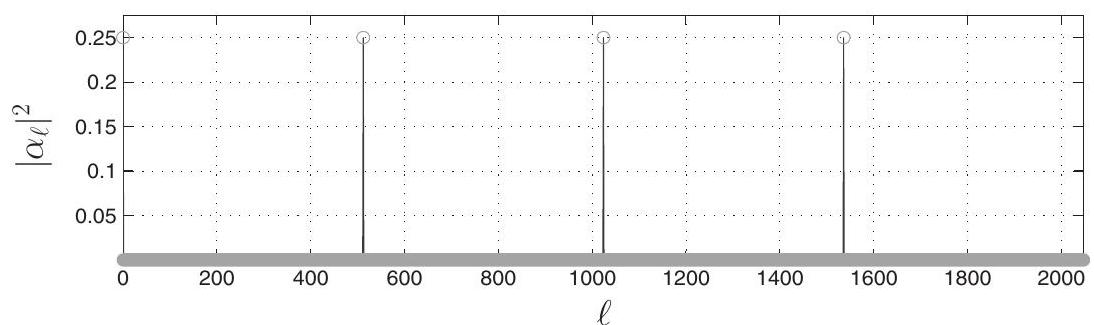
\includegraphics[width=0.75\linewidth]{Images/2024_05_17_6977ce60de6fd27aef98g-269}
\end{figure}

shown for $2^{t}=2048$. The final measurement therefore gives either $0,512,1024$, or 1536 , each with probability almost exactly $1 / 4$. Suppose we obtain $\ell=1536$ from the measurement; computing the continued fraction expansion thus gives $1536 / 2048=1 /(1+(1 / 3))$, so that $3 / 4$ occurs as a convergent in the expansion, giving $r=4$ as the order of $x=7$. By chance, $r$ is even, and moreover, $x^{r / 2} \bmod N=7^{2} \bmod 15=4 \neq-1 \bmod 15$, so the algorithm works: computing the greatest common divisor $\operatorname{gcd}\left(x^{2}-1,15\right)=3$ and $\operatorname{gcd}\left(x^{2}+1,15\right)=5$ tells us that $15=3 \times 5$.\\
of the function may be very intricate. In order to present this problem in the most approachable manner, we begin with two more specific applications: period-finding (of a one-dimensional function), and discrete logarithms. We then return to the general hidden subgroup problem. Note that the presentation in this section is rather more schematic and conceptual than earlier sections in this chapter; of necessity, this means that the reader interested in understanding all the details will have to work much harder!

\subsection{5.4.1 Period-finding}
Consider the following problem. Suppose $f$ is a periodic function producing a single bit as output and such that $f(x+r)=f(x)$, for some unknown $0<r<2^{L}$, where $x, r \in\{0,1,2, \ldots\}$. Given a quantum black box $U$ which performs the unitary transform $U|x\rangle|y\rangle \rightarrow|x\rangle|y \oplus f(x)\rangle$ (where $\oplus$ denotes addition modulo 2) how many black box queries and other operations are required to determine $r$ ? Note that in practice $U$ operates on a finite domain, whose size is determined by the desired accuracy for $r$. Here is a quantum algorithm which solves this problem using one query, and $O\left(L^{2}\right)$ other operations:

\textbf{Algorithm: Period-finding}
Inputs: (1) A black box which performs the operation $U|x\rangle|y\rangle=|x\rangle|y \oplus f(x)\rangle$, (2) a state to store the function evaluation, initialized to $|0\rangle$, and (3) $t=O(L+\log (1 / \epsilon))$ qubits initialized to $|0\rangle$.

Outputs: The least integer $r>0$ such that $f(x+r)=f(x)$.

Runtime: One use of $U$, and $O\left(L^{2}\right)$ operations. Succeeds with probability $O(1)$.

\textbf{Procedure:}
\begin{enumerate}
    \item $\quad|0\rangle|0\rangle$
    \item $\rightarrow \frac{1}{\sqrt{2^{t}}} \sum_{x=0}^{2^{t}-1}|x\rangle|0\rangle$
    \item $\rightarrow \frac{1}{\sqrt{2^{t}}} \sum_{x=0}^{2^{t}-1}|x\rangle|f(x)\rangle$

\end{enumerate}

$\approx \frac{1}{\sqrt{r 2^{t}}} \sum_{\ell=0}^{r-1} \sum_{x=0}^{2^{t}-1} e^{2 \pi i \ell x / r}|x\rangle|\hat{f}(\ell)\rangle$

\begin{enumerate}
  \setcounter{enumi}{3}
    \item $\left.\quad \rightarrow \frac{1}{\sqrt{r}} \sum_{\ell=0}^{r-1}|\widetilde{\ell / r\rangle}| \hat{f}(\ell)\right\rangle$
    \item $\quad \rightarrow \widetilde{\ell / r}$
    \item $\rightarrow r$ initial state

\end{enumerate}

create superposition

apply $U$

apply inverse Fourier transform to first register

measure first register

apply continued fractions algorithm

The key to understanding this algorithm, which is based on phase estimation, and is nearly identical to the algorithm for quantum order-finding, is step 3 , in which we introduce the state

\begin{equation}
    |\hat{f}(\ell)\rangle \equiv \frac{1}{\sqrt{r}} \sum_{x=0}^{r-1} e^{-2 \pi i \ell x / r}|f(x)\rangle \tag{5.63}
\end{equation}

the Fourier transform of $|f(x)\rangle$. The identity used in step 3 is based on

\begin{equation}
    |f(x)\rangle=\frac{1}{\sqrt{r}} \sum_{\ell=0}^{r-1} e^{2 \pi i \ell x / r}|\hat{f}(\ell)\rangle \tag{5.64}
\end{equation}

which is easy to verify by noting that $\sum_{\ell=0}^{r-1} e^{2 \pi i \ell x / r}=r$ for $x$ an integer multiple of $r$, and zero otherwise. The approximate equality in step 3 is required because $2^{t}$ may not be an integer multiple of $r$ in general (it need not be: this is taken account of by the phase estimation bounds). By Equation (5.22), applying the inverse Fourier transform to the first register, in step 4 , gives an estimate of the phase $\ell / r$, where $\ell$ is chosen randomly. $r$ can be efficiently obtained in the final step using a continued fraction expansion.

\textbf{Box5.5: The shift-invariance property of the Fourier transform}
The Fourier transform, Equation (5.1), has an interesting and very useful property, known as shift invariance. Using notation which is useful in describing the general application of this property, let us describe the quantum Fourier transform as

\begin{equation}
    \sum_{h \in H} \alpha_{h}|h\rangle \rightarrow \sum_{g \in G} \tilde{\alpha}_{g}|g\rangle, \tag{5.65}
\end{equation}

where $\tilde{\alpha}_{g}=\sum_{h \in H} \alpha_{h} \exp (2 \pi i g h /|G|), H$ is some subset of $G$, and $G$ indexes the states in an orthonormal basis of the Hilbert space. For example, $G$ may be the set of numbers from 0 to $2^{n}-1$ for an $n$ qubit system. $|G|$ denotes the number of elements in $G$. Suppose we apply to the initial state an operator $U_{k}$ which performs the unitary transform

\begin{equation}
    U_{k}|g\rangle=|g+k\rangle, \tag{5.66}
\end{equation}

then apply the Fourier transform. The result,

\begin{equation}
    U_{k} \sum_{h \in H} \alpha_{h}|h\rangle=\sum_{h \in H} \alpha_{h}|h+k\rangle \rightarrow \sum_{g \in G} e^{2 \pi i g k /|G|} \tilde{\alpha}_{g}|g\rangle \tag{5.67}
\end{equation}

has the property that the magnitude of the amplitude for $|g\rangle$ does not change, no matter what $k$ is, that is: $\left|\exp (2 \pi i g k /|G|) \tilde{\alpha}_{g}\right|=\left|\tilde{\alpha}_{g}\right|$.

In the language of group theory, $G$ is a group, $H$ a subgroup of $G$, and we say that if a function $f$ on $G$ is constant on cosets of $H$, then the Fourier transform of $f$ is invariant over cosets of $H$.

Why does this work? One way to understand this is to realize that (5.63) is approximately the Fourier transform over $\left\{0,1, \ldots, 2^{L}-1\right\}$ of $|f(x)\rangle$ (see Exercise 5.20), and the Fourier transform has an interesting and very useful property, known as shift invariance, described in Box 5.5. Another is to realize that what the order-finding algorithm does is just to find the period of the function $f(k)=x^{k} \bmod N$, so the ability to find the period of a general periodic function is not unexpected. Yet another way is to realize that the implementation of the black box $U$ is naturally done using a certain unitary operator whose eigenvectors are precisely $|\hat{f}(\ell)\rangle$, as described in Exercise 5.21 below, so that the phase estimation procedure of Section 5.2 can be applied.

Exercise 5.20: Suppose $f(x+r)=f(x)$, and $0 \leq x<N$, for $N$ an integer multiple of $r$. Compute

\begin{equation}
    \hat{f}(\ell) \equiv \frac{1}{\sqrt{N}} \sum_{x=0}^{N-1} e^{-2 \pi i \ell x / N} f(x) \tag{5.68}
\end{equation}

and relate the result to (5.63). You will need to use the fact that

\begin{equation}
    \sum_{k \in\{0, r, 2 r, \ldots, N-r\}} e^{2 \pi i k \ell / N}= \begin{cases}\sqrt{N / r} & \text { if } \ell \text { is an integer multiple of } N / r  \tag{5.69}\\ 0 & \text { otherwise. }\end{cases}
\end{equation}

Exercise 5.21: (Period-finding and phase estimation) Suppose you are given a unitary operator $U_{y}$ which performs the transformation $U_{y}|f(x)\rangle=|f(x+y)\rangle$, for the periodic function described above.

(1) Show that the eigenvectors of $U_{y}$ are $|\hat{f}(\ell)\rangle$, and calculate their eigenvalues.

(2) Show that given $\left|f\left(x_{0}\right)\right\rangle$ for some $x_{0}, U_{y}$ can be used to realize a black box which is as useful as $U$ in solving the period-finding problem.

\subsection{5.4.2 Discrete Logarithms}
The period finding problem we just considered is a simple one, in that the domain and range of the periodic function were integers. What happens when the function is more complex? Consider the function $f\left(x_{1}, x_{2}\right)=a^{s x_{1}+x_{2}} \bmod N$, where all the variables are integers, and $r$ is the smallest positive integer for which $a^{r} \bmod N=1$. This function is periodic, since $f\left(x_{1}+\ell, x_{2}-\ell s\right)=f\left(x_{1}, x_{2}\right)$, but now the period is a 2-tuple, $(\ell,-\ell s)$, for integer $\ell$. This may seem to be a strange function, but it is very useful in cryptography, since determining $s$ allows one to solve what is known as the discrete logarithm problem: given $a$ and $b=a^{s}$, what is $s$ ? Here is a quantum algorithm which solves this problem using one query of a quantum black box $U$ which performs the unitary transform $U\left|x_{1}\right\rangle\left|x_{2}\right\rangle|y\rangle \rightarrow\left|x_{1}\right\rangle\left|x_{2}\right\rangle|y \oplus f(x)\rangle($ where $\oplus$ denotes bitwise addition modulo 2), and $O\left(\lceil\log r\rceil^{2}\right)$ other operations. We assume knowledge of the minimum $r>0$ such that $a^{r} \bmod N=1$, which can be obtained using the order-finding algorithm described previously.

\textbf{Algorithm: Discrete logarithm}
Inputs: (1) A black box which performs the operation

$U\left|x_{1}\right\rangle\left|x_{2}\right\rangle|y\rangle=\left|x_{1}\right\rangle\left|x_{2}\right\rangle\left|y \oplus f\left(x_{1}, x_{2}\right)\right\rangle$, for $f\left(x_{1}, x_{2}\right)=b^{x_{1}} a^{x_{2}},(2)$ a state to store the function evaluation, initialized to $|0\rangle$, and (3) two $t=O(\lceil\log r\rceil+\log (1 / \epsilon))$ qubit registers initialized to $|0\rangle$.

Outputs: The least positive integer $s$ such that $a^{s}=b$.

Runtime: One use of $U$, and $O\left(\lceil\log r\rceil^{2}\right)$ operations. Succeeds with probability $O(1)$.

\textbf{Procedure:}
\begin{enumerate}
    \item $\quad|0\rangle|0\rangle|0\rangle$
\end{enumerate}

initial state\\
2. $\quad \rightarrow \frac{1}{2^{t}} \sum_{x_{1}=0}^{2^{t}-1} \sum_{x_{2}=0}^{2^{t}-1}\left|x_{1}\right\rangle\left|x_{2}\right\rangle|0\rangle \quad$ create superposition\\
3. $\quad \rightarrow \frac{1}{2^{t}} \sum_{x_{1}=0}^{2^{t}-1} \sum_{x_{2}=0}^{2^{t}-1}\left|x_{1}\right\rangle\left|x_{2}\right\rangle\left|f\left(x_{1}, x_{2}\right)\right\rangle \quad$ apply $U$ $\approx \frac{1}{2^{t} \sqrt{r}} \sum_{\ell_{2}=0}^{r-1} \sum_{x_{1}=0}^{2^{t}-1} \sum_{x_{2}=0}^{2^{t}-1} e^{2 \pi i\left(s \ell_{2} x_{1}+\ell_{2} x_{2}\right) / r}\left|x_{1}\right\rangle\left|x_{2}\right\rangle\left|\hat{f}\left(s \ell_{2}, \ell_{2}\right)\right\rangle$ $=\frac{1}{2^{t} \sqrt{r}} \sum_{\ell_{2}=0}^{r-1}\left[\sum_{x_{1}=0}^{2^{t}-1} e^{2 \pi i\left(s \ell_{2} x_{1}\right) / r}\left|x_{1}\right\rangle\right]\left[\sum_{x_{2}=0}^{2^{t}-1} e^{2 \pi i\left(\ell_{2} x_{2}\right) / r}\left|x_{2}\right\rangle\right]\left|\hat{f}\left(s \ell_{2}, \ell_{2}\right)\right\rangle$\\
4. $\left.\quad \rightarrow \frac{1}{\sqrt{r}} \sum_{\ell_{2}=0}^{r-1}\left|\widetilde{\ell_{2} / r} r\right| \widetilde{\ell_{2} / r}\right\rangle\left|\hat{f}\left(s \ell_{2}, \ell_{2}\right)\right\rangle \quad$ apply inverse Fourier transform to first\\
5. $\rightarrow\left(\widetilde{s \ell_{2} / r}, \widetilde{\ell_{2} / r}\right) \quad$ measure first two registers\\
6. $\quad \rightarrow s$

apply generalized continued fractions algorithm

Again, the key to understanding this algorithm is step 3 , in which we introduce the state

\begin{equation}
    \left|\hat{f}\left(\ell_{1}, \ell_{2}\right)\right\rangle=\frac{1}{\sqrt{r}} \sum_{j=0}^{r-1} e^{-2 \pi i \ell_{2} j / r}|f(0, j)\rangle \tag{5.70}
\end{equation}

the Fourier transform of $\left|f\left(x_{1}, x_{2}\right)\right\rangle$ (see Exercise 5.22). In this equation, the values of $\ell_{1}$ and $\ell_{2}$ must satisfy

\begin{equation}
    \sum_{k=0}^{r-1} e^{2 \pi i k\left(\ell_{1} / s-\ell_{2}\right) / r}=r \tag{5.71}
\end{equation}

Otherwise, the amplitude of $\left|\hat{f}\left(\ell_{1}, \ell_{2}\right)\right\rangle$ is nearly zero. The generalized continued fraction expansion used in the final step to determine $s$ is analogous to the procedures used in Section 5.3.1, and is left as a simple exercise for you to construct.

Exercise 5.22: Show that

\begin{equation}
    \left|\hat{f}\left(\ell_{1}, \ell_{2}\right)\right\rangle=\sum_{x_{1}=0}^{r-1} \sum_{x_{2}=0}^{r-1} e^{-2 \pi i\left(\ell_{1} x_{1}+\ell_{2} x_{2}\right) / r}\left|f\left(x_{1}, x_{2}\right)\right\rangle=\frac{1}{\sqrt{r}} \sum_{j=0}^{r-1} e^{-2 \pi i \ell_{2} j / r}|f(0, j)\rangle \tag{5.72}
\end{equation}

and we are constrained to have $\ell_{1} / s-\ell_{2}$ be an integer multiple of $r$ for this expression to be non-zero.

Exercise 5.23: Compute

\begin{equation}
    \frac{1}{r} \sum_{\ell_{1}=0}^{r-1} \sum_{\ell_{2}=0}^{r-1} e^{-2 \pi i\left(\ell_{1} x_{1}+\ell_{2} x_{2}\right) / r}\left|\hat{f}\left(\ell_{1}, \ell_{2}\right)\right\rangle \tag{5.73}
\end{equation}

using (5.70), and show that the result is $f\left(x_{1}, x_{2}\right)$.

Exercise 5.24: Construct the generalized continued fractions algorithm needed in\\
step 6 of the discrete logarithm algorithm to determine $s$ from estimates of $s \ell_{2} / r$ and $\ell_{2} / r$.

Exercise 5.25: Construct a quantum circuit for the black box $U$ used in the quantum discrete logarithm algorithm, which takes $a$ and $b$ as parameters, and performs the unitary transform $\left|x_{1}\right\rangle\left|x_{2}\right\rangle|y\rangle \rightarrow\left|x_{1}\right\rangle\left|x_{2}\right\rangle\left|y \oplus b^{x_{1}} a^{x_{2}}\right\rangle$. How many elementary operations are required?

\subsection{5.4.3 The Hidden Subgroup Problem}
By now, a pattern should be coming clear: if we are given a periodic function, even when the structure of the periodicity is quite complicated, we can often use a quantum algorithm to determine the period efficiently. Importantly, however, not all periods of periodic functions can be determined. The general problem which defines a broad framework for these questions can be succinctly expressed in the language of group theory (see Appendix 2 for a quick review) as follows:

Let $f$ be a function from a finitely generated group $G$ to a finite set $X$ such that $f$ is constant on the cosets of a subgroup $K$, and distinct on each coset. Given a quantum black box for performing the unitary transform $U|g\rangle|h\rangle=|g\rangle|h \oplus f(g)\rangle$, for $g \in G, h \in X$, and $\oplus$ an appropriately chosen binary operation on $X$, find a generating set for $K$.

Order-finding, period-finding, discrete logarithms, and many other problems are instances of this hidden subgroup problem; some interesting ones are listed in Figure 5.5.

For $G$ a finite Abelian group, a quantum computer can solve the hidden subgroup problem using a number of operations polynomial in $\log |G|$, and one use of the black box function evaluation, using an algorithm very similar to the others in this section. (In fact, solution for a finitely generated Abelian group is also possible, along similar lines, but we'll stick to the finite case here.) We shall leave detailed specification of the algorithm to you as an exercise, which should be simple after we explain the basic idea. Many things remain essentially the same, because finite Abelian groups are isomorphic to products of additive groups over the integers in modular arithmetic. This means that the quantum Fourier transform of $f$ over $G$ is well defined (see Section A2.3), and can still be done efficiently. The first non-trivial step of the algorithm is to use a Fourier transform (generalizing the Hadamard operation) to create a superposition over group elements, which is then transformed by applying the quantum black box for $f$ in the next step, to give

\begin{equation}
    \frac{1}{\sqrt{|G|}} \sum_{g \in G}|g\rangle|f(g)\rangle \tag{5.74}
\end{equation}

As before, we would now like to rewrite $|f(g)\rangle$ in the Fourier basis. We start with

\begin{equation}
    |f(g)\rangle=\frac{1}{\sqrt{|G|}} \sum_{\ell=0}^{|G|-1} e^{2 \pi i \ell g /|G|}|\hat{f}(\ell)\rangle \tag{5.75}
\end{equation}

where we have chosen $\exp [-2 \pi i \ell g /|G|]$ as a representation (see Exercise A2.13) of $g \in G$ indexed by $\ell$ (the Fourier transform maps between group elements and representations: see Exercise A2.23). The key is to recognize that this expression can be simplified because

\begin{center}
\begin{tabular}{|c|c|c|c|c|}
\hline
Name & $G$ & $X$ & K & Function \\
\hline
Deutsch & $\{0,1\}, \oplus$ & $\{0,1\}$ & $\{0\}$ or $\{0,1\}$ & \begin{tabular}{l}
$K=\{0,1\}:\left\{\begin{array}{l}f(x)=0 \\ f(x)=1\end{array}\right.$ \\
$K=\{0\}:\left\{\begin{array}{l}f(x)=x \\ f(x)=1-x\end{array}\right.$ \\
\end{tabular} \\
\hline
Simon & $\{0,1\}^{n}, \oplus$ & \begin{tabular}{l}
any \\
finite \\
set \\
\end{tabular} & \begin{tabular}{c}
$\{0, s\}$ \\
$s \in\{0,1\}^{n}$ \\
\end{tabular} & $f(x \oplus s)=f(x)$ \\
\hline
\begin{tabular}{l}
Period- \\
finding \\
\end{tabular} & $\mathrm{Z},++$ & \begin{tabular}{l}
any \\
finite \\
set \\
\end{tabular} & \begin{tabular}{l}
$\{0, r, 2 r, \ldots\}$ \\
$\quad r \in G$ \\
\end{tabular} & $f(x+r)=f(x)$ \\
\hline
\begin{tabular}{l}
Order- \\
finding \\
\end{tabular} & $\mathrm{Z},+$ & \begin{tabular}{l}
$\left\{a^{j}\right\}$ \\
$j \in Z_{r}$ \\
$a^{r}=1$ \\
\end{tabular} & \begin{tabular}{c}
$\{0, r, 2 r, \ldots\}$ \\
$r \in G$ \\
\end{tabular} & \begin{tabular}{l}
$f(x)=a^{x}$ \\
$f(x+r)=f(x)$ \\
\end{tabular} \\
\hline
\begin{tabular}{l}
Discrete \\
logarithm \\
\end{tabular} & \begin{tabular}{c}
$\mathbf{Z}_{r} \times \mathbf{Z}_{r}$ \\
$+(\bmod r)$ \\
\end{tabular} & \begin{tabular}{l}
$\left\{a^{j}\right\}$ \\
$j \in Z_{r}$ \\
$a^{r}=1$ \\
\end{tabular} & \begin{tabular}{l}
$(\ell,-\ell s)$ \\
$\ell, s \in \mathbf{Z}_{r}$ \\
\end{tabular} & \begin{tabular}{l}
$f\left(x_{1}, x_{2}\right)=a^{k x_{1}+x_{2}}$ \\
$f\left(x_{1}+\ell, x_{2}-\ell s\right)=f\left(x_{1}, x_{2}\right)$ \\
\end{tabular} \\
\hline
\begin{tabular}{l}
Order of a \\
permutation \\
\end{tabular} & \begin{tabular}{l}
$\mathbf{Z}_{2^{m}} \times \mathbf{Z}_{2^{n}}$ \\
$+\left(\bmod 2^{m}\right)$ \\
\end{tabular} & $\mathbf{Z}_{2^{n}}$ & \begin{tabular}{l}
$\{0, r, 2 r, \ldots\}$ \\
$\quad r \in X$ \\
\end{tabular} & \begin{tabular}{l}
$f(x, y)=\pi^{x}(y)$ \\
$f(x+r, y)=f(x, y)$ \\
$\pi=$ permutation on $X$ \\
\end{tabular} \\
\hline
\begin{tabular}{l}
Hidden \\
linear \\
function \\
\end{tabular} & $\mathbf{Z} \times \mathbf{Z},+$ & $\mathbf{Z}_{N}$ & \begin{tabular}{l}
$(\ell,-\ell s)$ \\
$\ell, s \in X$ \\
\end{tabular} & \begin{tabular}{l}
$f\left(x_{1}, x_{2}\right)=$ \\
$\quad \pi\left(s x_{1}+x_{2} \bmod N\right)$ \\
$\pi=$ permutation on $X$ \\
\end{tabular} \\
\hline
\begin{tabular}{l}
Abelian \\
stabilizer \\
\end{tabular} & \begin{tabular}{l}
$(H, X)$ \\
$H=$ any \\
Abelian \\
group \\
\end{tabular} & \begin{tabular}{l}
any \\
finite \\
set \\
\end{tabular} & \begin{tabular}{l}
$\{s \in H \mid$ \\
$f(s, x)=x$ \\
$\forall x \in X\}$ \\
\end{tabular} & \begin{tabular}{l}
$f(g h, x)=f(g, f(h, x))$ \\
$f(g s, x)=f(g, x)$ \\
\end{tabular} \\
\hline
\end{tabular}
\end{center}

Figure 5.5. Hidden subgroup problems. The function $f$ maps from the group $G$ to the finite set $X$, and is promised to be constant on cosets of the hidden subgroup $K \subseteq G . \mathbf{Z}_{N}$ represents the set $\{0,1, \ldots, N-1\}$ in this table, and $\mathbf{Z}$ is the integers. The problem is to find $K$ (or a generating set for it), given a black box for $f$.

$f$ is constant and distinct on cosets of the subgroup $K$, so that

\begin{equation}
    |\hat{f}(\ell)\rangle=\frac{1}{\sqrt{|G|}} \sum_{g \in G} e^{-2 \pi i \ell g /|G|}|f(g)\rangle \tag{5.76}
\end{equation}

has nearly zero amplitude for all values of $\ell$ except those which satisfy

\begin{equation}
    \sum_{h \in K} e^{-2 \pi i \ell h /|G|}=|K| \tag{5.77}
\end{equation}

If we can determine $\ell$, then using the linear constraints given by this expression allows us to determine elements of $K$, and since $K$ is Abelian, this allows us to eventually determine a generating set for the whole hidden subgroup, solving the problem.

However, life is not so simple. An important reason why the period-finding and discrete logarithm algorithms work is because of the success of the continued fraction expansion in obtaining $\ell$ from $\ell /|G|$. In those problems, $\ell$ and $|G|$ are arranged to not have any common factors, with high probability. In the general case, however, this may not be true, since $|G|$ is free to be a composite number with many factors, and we have no useful prior information about $\ell$.

Fortunately, this problem can be solved: as mentioned above, any finite Abelian group $G$ is isomorphic to a product of cyclic groups of prime power order, that is, $G=\mathbf{Z}_{p_{1}} \times$ $\mathbf{Z}_{p_{2}} \times \cdots \times \mathbf{Z}_{p_{M}}$, where $p_{i}$ are primes, and $\mathbf{Z}_{p_{i}}$ is the group over integers $\left\{0,1, \ldots, p_{i}-1\right\}$ with addition modulo $p_{i}$ being the group operation. We can thus re-express the phase which appears in $(5.75)$ as

\begin{equation}
    e^{2 \pi i \ell g /|G|}=\prod_{i=1}^{M} e^{2 \pi i \ell_{i}^{\prime} g_{i} / p_{i}} \tag{5.78}
\end{equation}

for $g_{i} \in \mathbf{Z}_{p_{i}}$. The phase estimation procedure now gives us $\ell_{i}^{\prime}$, from which we determine $\ell$, and thus, sample $K$ as described above, to solve the hidden subgroup problem.

Exercise 5.26: $\quad$ Since $K$ is a subgroup of $G$, when we decompose $G$ into a product of cyclic groups of prime power order, this also decomposes $K$. Re-express (5.77) to show that determining $\ell_{i}^{\prime}$ allows one to sample from the corresponding cyclic subgroup $K_{p_{i}}$ of $K$.

Exercise 5.27: Of course, the decomposition of a general finite Abelian group $G$ into a product of cyclic groups of prime power order is usually a difficult problem (at least as hard as factoring integers, for example). Here, quantum algorithms come to the rescue again: explain how the algorithms in this chapter can be used to efficiently decompose $G$ as desired.

Exercise 5.28: Write out a detailed specification of the quantum algorithm to solve the hidden subgroup problem, complete with runtime and success probability estimates, for finite Abelian groups.

Exercise 5.29: Give quantum algorithms to solve the Deutsch and Simon problems listed in Figure 5.5, using the framework of the hidden subgroup problem.

\subsection{5.4.4 Other Quantum Algorithms?}
One of the most intriguing aspects of this framework for describing quantum algorithms in terms of the hidden subgroup problem is the suggestion that more difficult problems might be solvable by considering various groups $G$ and functions $f$. We have only described the solution of this problem for Abelian groups. What about non-Abelian groups? They are quite interesting (see Appendix 2 for a discussion of general Fourier transforms over non-Abelian groups): for example, the problem of graph isomorphism is to determine if two given graphs are the same under some permutation of the labels of the $n$ vertices (Section 3.2.3). These permutations can be described as transformations under the symmetric group $S_{n}$, and algorithms for performing fast Fourier transforms\\
over these groups exists. However, a quantum algorithm for efficiently solving the graph isomporphism problem remains unknown.

Even if more general cases of the hidden subgroup problem remain unsolvable by quantum computers, having this unifying framework is useful, because it allows us to ask questions about how one might be able to step outside its limitations. It is difficult to believe that all fast quantum algorithms that will ever be discovered will be just ways to solve the hidden subgroup problem. If one thinks of these problems as being based on the coset invariance property of the Fourier transform, in searching for new algorithms, perhaps the thing to do then is to investigate other transforms with different invariances. Going in another direction, one might ask: what difficult hidden subgroup problems might be efficiently solved given an arbitrary (but specified independently of the problem) quantum state as a helper? After all, as discussed in Chapter 4, most quantum states are actually exponentially hard to construct. Such a state might be a useful resource (a real 'quantum oracle'), if quantum algorithms existed to utilize them to solve hard problems!

The hidden subgroup problem also captures an important constraint underlying the class of quantum algorithms which are exponentially faster than their (known) classical counterparts: this is a promise problem, meaning that it is of the form ' $F(X)$ is promised to have such and such property: characterize that property.' Rather disappointingly, perhaps, we shall show at the end of the next chapter that, in solving problems without some sort of promise, quantum computers cannot achieve an exponential speedup over classical computers; the best speedup is polynomial. On the other hand, this gives us an important clue as to what kinds of problems quantum computers might be good at: in retrospect, the hidden subgroup problem might be thought of as a natural candidate for quantum computation. What other natural problems are there? Think about it!

Problem 5.1: Construct a quantum circuit to perform the quantum Fourier transform

\begin{equation}
    |j\rangle \longrightarrow \frac{1}{\sqrt{p}} \sum_{k=0}^{p-1} e^{2 \pi i j k / p}|k\rangle \tag{5.79}
\end{equation}

where $p$ is prime.

Problem 5.2: (Measured quantum Fourier transform) Suppose the quantum Fourier transform is performed as the last step of a quantum computation, followed by a measurement in the computational basis. Show that the combination of quantum Fourier transform and measurement is equivalent to a circuit consisting entirely of one qubit gates and measurement, with classical control, and no two qubit gates. You may find the discussion of Section 4.4 useful.

Problem 5.3: (Kitaev's algorithm) Consider the quantum circuit

\begin{figure}
\centering
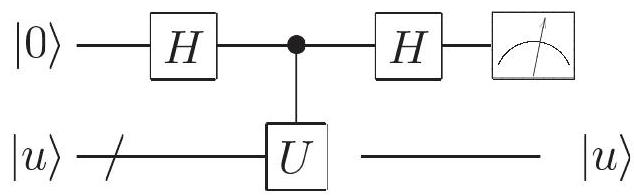
\includegraphics[width=0.75\linewidth]{Images/2024_05_17_6977ce60de6fd27aef98g-277}
\end{figure}

where $|u\rangle$ is an eigenstate of $U$ with eigenvalue $e^{2 \pi i \varphi}$. Show that the top qubit is\\
measured to be 0 with probability $p \equiv \cos ^{2}(\pi \varphi)$. Since the state $|u\rangle$ is unaffected by the circuit it may be reused; if $U$ can be replaced by $U^{k}$, where $k$ is an arbitrary integer under your control, show that by repeating this circuit and increasing $k$ appropriately, you can efficiently obtain as many bits of $p$ as desired, and thus, of $\varphi$. This is an alternative to the phase estimation algorithm.

Problem 5.4: The runtime bound $O\left(L^{3}\right)$ we have given for the factoring algorithm is not tight. Show that a better upper bound of $O\left(L^{2} \log L \log \log L\right)$ operations can be achieved.

Problem 5.5: (Non-Abelian hidden subgroups - Research) Let $f$ be a function on a finite group $G$ to an arbitrary finite range $X$, which is promised to be constant and distinct on distinct left cosets of a subgroup $K$. Start with the state

\begin{equation}
    \frac{1}{\sqrt{|G|^{m}}} \sum_{g_{1}, \ldots, g_{m}}\left|g_{1}, \ldots, g_{m}\right\rangle\left|f\left(g_{1}\right), \ldots, f\left(g_{m}\right)\right\rangle \tag{5.80}
\end{equation}

and prove that picking $m=4 \log |G|+2$ allows $K$ to be identified with probability at least $1-1 /|G|$. Note that $G$ does not necessarily have to be Abelian, and being able to perform a Fourier transform over $G$ is not required. This result shows that one can produce (using only $O(\log |G|)$ oracle calls) a final result in which the pure state outcomes corresponding to different possible hidden subgroups are nearly orthogonal. However, it is unknown whether a POVM exists or not which allows the hidden subgroup to be identified efficiently (i.e. using poly $(\log |G|)$ operations) from this final state.

Problem 5.6: (Addition by Fourier transforms) Consider the task of constructing a quantum circuit to compute $|x\rangle \rightarrow\left|x+y \bmod 2^{n}\right\rangle$, where $y$ is a fixed constant, and $0 \leq x<2^{n}$. Show that one efficient way to do this, for values of $y$ such as 1, is to first perform a quantum Fourier transform, then to apply single qubit phase shifts, then an inverse Fourier transform. What values of $y$ can be added easily this way, and how many operations are required?

Summary of Chapter 5: The quantum Fourier transform and its applications

\begin{itemize}
    \item When $N=2^{n}$ the quantum Fourier transform
\end{itemize}

\begin{equation}
    |j\rangle=\left|j_{1}, \ldots, j_{n}\right\rangle \longrightarrow \frac{1}{\sqrt{N}} \sum_{k=0}^{N-1} e^{2 \pi i \frac{i k}{N}}|k\rangle \tag{5.81}
\end{equation}

may be written in the form

\begin{equation}
    |j\rangle \rightarrow \frac{1}{2^{n / 2}}\left(|0\rangle+e^{2 \pi i 0 \cdot j_{n}}|1\rangle\right)\left(|0\rangle+e^{2 \pi i 0 \cdot j_{n-1} j_{n}}|1\rangle\right) \ldots\left(|0\rangle+e^{2 \pi i 0 \cdot j_{1} j_{2} \ldots j_{n}}|1\rangle\right) \tag{5.82}
\end{equation}

and may be implemented using $\Theta\left(n^{2}\right)$ gates.

\begin{itemize}
    \item Phase estimation: Let $|u\rangle$ be an eigenstate of the operator $U$ with eigenvalue $e^{2 \pi i \varphi}$. Starting from the initial state $|0\rangle^{\otimes t}|u\rangle$, and given the ability to efficiently perform $U^{2^{k}}$ for integer $k$, this algorithm (shown in Figure 5.3) can be used to efficiently obtain the state $|\tilde{\varphi}\rangle|u\rangle$, where $\tilde{\varphi}$ accurately approximates $\varphi$ to $t-$ $\left\lceil\log \left(2+\frac{1}{2 \epsilon}\right)\right\rceil$ bits with probability at least $1-\epsilon$.
    \item Order-finding: The order of $x$ modulo $N$ is the least positive integer $r$ such that $x^{r} \bmod N=1$. This number can be computed in $O\left(L^{3}\right)$ operations using the quantum phase estimation algorithm, for $L$-bit integers $x$ and $N$.
    \item Factoring: The prime factors of an $L$-bit integer $N$ can be determined in $O\left(L^{3}\right)$ operations by reducing this problem to finding the order of a random number $x$ co-prime with $N$.
    \item Hidden subgroup problem: All the known fast quantum algorithms can be described as solving the following problem: Let $f$ be a function from a finitely generated group $G$ to a finite set $X$ such that $f$ is constant on the cosets of a subgroup $K$, and distinct on each coset. Given a quantum black box for performing the unitary transform $U|g\rangle|h\rangle=|g\rangle|h \oplus f(g)\rangle$, for $g \in G$ and $h \in X$, find a generating set for $K$.
\end{itemize}

\section{History and Further Reading}
The definition of the Fourier transform may be generalized beyond what we have considered in this chapter. In the general scenario a Fourier transform is defined on a set of complex numbers $\alpha_{g}$, where the index $g$ is chosen from some group, $G$. In this chapter we have chosen $G$ to be the additive group of integers modulo $2^{n}$, often denoted $\mathbf{Z}_{2^{n}}$. Deutsch ${ }^{[\text {Deu85] }}$ showed that the Fourier transform over the group $\mathbf{Z}_{2}^{n}$ could be implemented efficiently on a quantum computer - this is the Hadamard transform of earlier chapters. Shor ${ }^{[S h o 94]}$ realized to spectacular effect that quantum computers could efficiently implement the quantum Fourier transform over groups $\mathbf{Z}_{m}$ for certain special values of $m$. Inspired by this result Coppersmith ${ }^{[\text {Coppy] }}$, Deutsch (unpublished), and Cleve (unpublished) gave the simple quantum circuits for computing the quantum Fourier transform over $\mathbf{Z}_{2^{n}}$ which we have used in this chapter. Cleve, Ekert, Mac-\\
chiavello and Mosca[CEMM98] and Griffiths and $\mathrm{Niu}^{[\mathrm{GN} 96]}$ independently discovered the product formula (5.4); in fact, this result had been realized much earlier by Danielson and Lanczos. The simplified proof starting in Equation (5.5) was suggested by Zhou. Griffiths and Niu ${ }^{[G N 96]}$ are responsible for the measured quantum Fourier transform found in Problem 5.2.

The Fourier transform over $\mathbf{Z}_{2^{n}}$ was generalized to obtain a Fourier transform over an arbitrary finite Abelian group by $\mathrm{Kitaev}^{[\mathrm{Kit} 95]}$, who also introduced the phase estimation procedure in the form given in Problem 5.3. Cleve, Ekert, Macchiavello and Mosca ${ }^{[C E M M 98]}$ also integrated several of the techniques of Shor and Kitaev into one nice picture, upon which Section 5.2 is based. A good description of the phase estimation algorithm can be found in Mosca's Ph.D. thesis ${ }^{[\text {Mos999] }}$.

Shor announced the quantum order-finding algorithm in a seminal paper in 1994 [Sho94], and noted that the problems of performing discrete logarithms and factoring could be reduced to order-finding. The final paper, including extended discussion and references, was published in $1997^{[\text {Sho } 07]}$. This paper also contains a discussion of clever multiplication methods that may be used to speed up the algorithm even further than in our description, which uses relatively naive multiplication techniques. With these faster multiplication methods the resources required to factor a composite integer $n$ scale as $O\left(n^{2} \log n \log \log n\right)$, as claimed in the introduction to the chapter. In $1995 \mathrm{Kitaev}^{[\mathrm{Kit} 95]}$ announced an algorithm for finding the stabilizer of a general Abelian group, which he showed could be used to solve discrete logarithm and factoring as special cases. In addition, this algorithm contained several elements not present in Shor's algorithm. A good review of the factoring algorithm was written by Ekert and Jozsa [E]96]; also see DiVincenzo [DiV95a]. The discussion of continued fractions is based upon Chapter 10 of Hardy and Wright ${ }^{[H W 60]}$. At the time of writing, the most efficient classical algorithm for factoring on a classical computer is the number field sieve. This is described in a collection edited by A. K. Lenstra and H. W. Lenstra, Jr.[LL93].

The generalization of quantum algorithms to solving the hidden subgroup problem has been considered by many authors. Historically, Simon was first to note that a quantum computer could find a hidden period of a function satisfying $f(x \oplus s)=f(x)^{[S i m 94, ~ S i m 97]}$. In fact, Shor found his result by generalizing Simon's result, and by applying a Fourier transform over $\mathbf{Z}_{N}$ instead of Simon's Hadamard transforms (a Fourier transform over $\mathbf{Z}_{2}^{k}$ ). Boneh and Lipton then noted the connection to the hidden subgroup problem, and described a quantum algorithm for solving the hidden linear function problem ${ }^{[B L 95]}$. Jozsa was the first to explicitly provide a uniform description of the Deutsch-Jozsa, Simon, and Shor algorithms in terms of the hidden subgroup problem ${ }^{[J o z 97]}$. Ekert and Jozsa's work in studying the role of the Abelian and non-Abelian Fast Fourier Transform algorithms in speedup of quantum algorithms $\mathrm{s}^{[\mathrm{E}] 98]}$ has also been insightful. Our description of the hidden subgroup problem in Section 5.4 follows the framework of Mosca and Ekert ${ }^{[\text {ME99, Mos99] }}$. Cleve has proven that the problem of finding an order of a permutation requires an exponential number of queries for a bounded-error probabilistic classical computer ${ }^{[\text {Cle99] }}$. Generalizations of this method to beyond Abelian groups have been attempted by Ettinger and Hoyer ${ }^{[\mathrm{EH} 99]}$, by Roetteler and Beth ${ }^{[\mathrm{RB} 98]}$ and Pueschel, Roetteler, and Beth ${ }^{[\text {PRB98] }}$, by Beals, who also described constructions of quantum Fourier

\begin{figure}
\centering
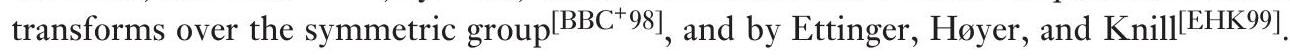
\includegraphics[width=0.75\textwidth]{Images/2024_05_17_6977ce60de6fd27aef98g-280}
\end{figure}

These results have shown, so far, that there exists a quantum algorithm to solve the hidden subgroup problem for non-Abelian groups using only $O(\log |G|)$ oracle calls, but whether this can be realized in polynomial time is unknown (Problem 5.5).

